\documentclass[a4paper,11pt]{article}
%\usepackage[T1]{fontenc}

%\setlength{\textwidth}{20cm}
%\setlength{\marginparwidth}{0cm}
%\setlength{\voffset}{0cm}
\usepackage[utf8]{inputenc}
\usepackage[francais]{babel}
\usepackage{amsmath}
\usepackage{graphicx}
\usepackage{listings}
%==== to fix locations of figures and tables
\usepackage{float}
\usepackage{placeins}

\lstset{
language=VHDL,
basicstyle=\small\sffamily,
numbers=left,
numberstyle=\tiny,
frame=tb,
columns=fullflexible,
showstringspaces=false
}
%\special{papersize=210mm,297mm}

\title{{\Huge Electronique numérique}\\Décomposition FSMD et Synthèse d'un système numérique}
%\title{TD1}
\date{}

\begin{document}
\maketitle

% ANNEE prochaine ==> load avec registre à décallage
\section{But du TE}

Le but de ce TE est de ``synthétiser'' un circuit numérique sur un FPGA. C'est la première expérience concrète que l'on réalise dans l'UV 1.5 ! \\

Nous allons pour cela procéder de la même manière qu'aux TE précédents, en adjoignant une nouvelle étape dans le processus :

\begin{itemize}
\item Formuler le problème sous forme de {\bf diagramme à bulles}.
\item Etablir les équations logique de notre {\bf contrôleur} \footnote { (ou ``FSM'' ou ``automate'',...)}
\item {\bf Simuler} le circuit virtuel pour s'assurer qu'il fonctionne comme prévu.
\item {\bf Synthétiser} le circuit sur FPGA, et le faire fonctionner ``pour de vrai''.
\end{itemize}

\section{Position du problème : multiplieur séquentiel}

Nous savons qu'il est {\it certes} possible de trouver un circuit purement {\it combinatoire} qui réalise la multiplication...Nous n'allons pas procéder ainsi.\\

Le multiplieur  proposé ici {\it séquentiel} : il lui faudra plusieurs cycles pour réaliser son calcul. L'algorithme de multiplication séquentielle reproduit ce que l'on fait sur papier, lorsqu'on multiplie 2 nombres.\\

Pour multiplier $X$ par $Y$, la methode consiste à cumuler séquentiellement les produits partiels :

$$ P=X \times Y = \sum_{i}Y_i\times X \times 2^i$$

Il est très important de comprendre la signification de cette équation : selon la valeur de $Y_i$, le terme $ (Y_i \times X) \times  2^i $ de rang i de la somme vaut :
\begin{itemize}
\item 0 si Yi = 0 ou
\item X décalé de i positions vers la gauche si $Yi = 1$. Le décallage se fait par $2^i$ !
\end{itemize}


\begin{figure}[!h]
\begin{center}
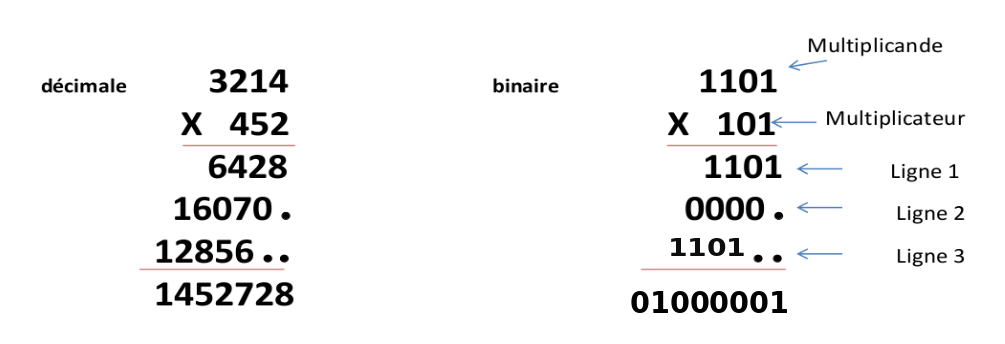
\includegraphics[scale=0.4]{./figures/algo_mult2.png}
\end{center}
\caption{Principe de la multiplication : une séquence de produits partiels et de décalages}
\end{figure}
%\FloatBarrier

\begin{figure}[!h]
\begin{center}
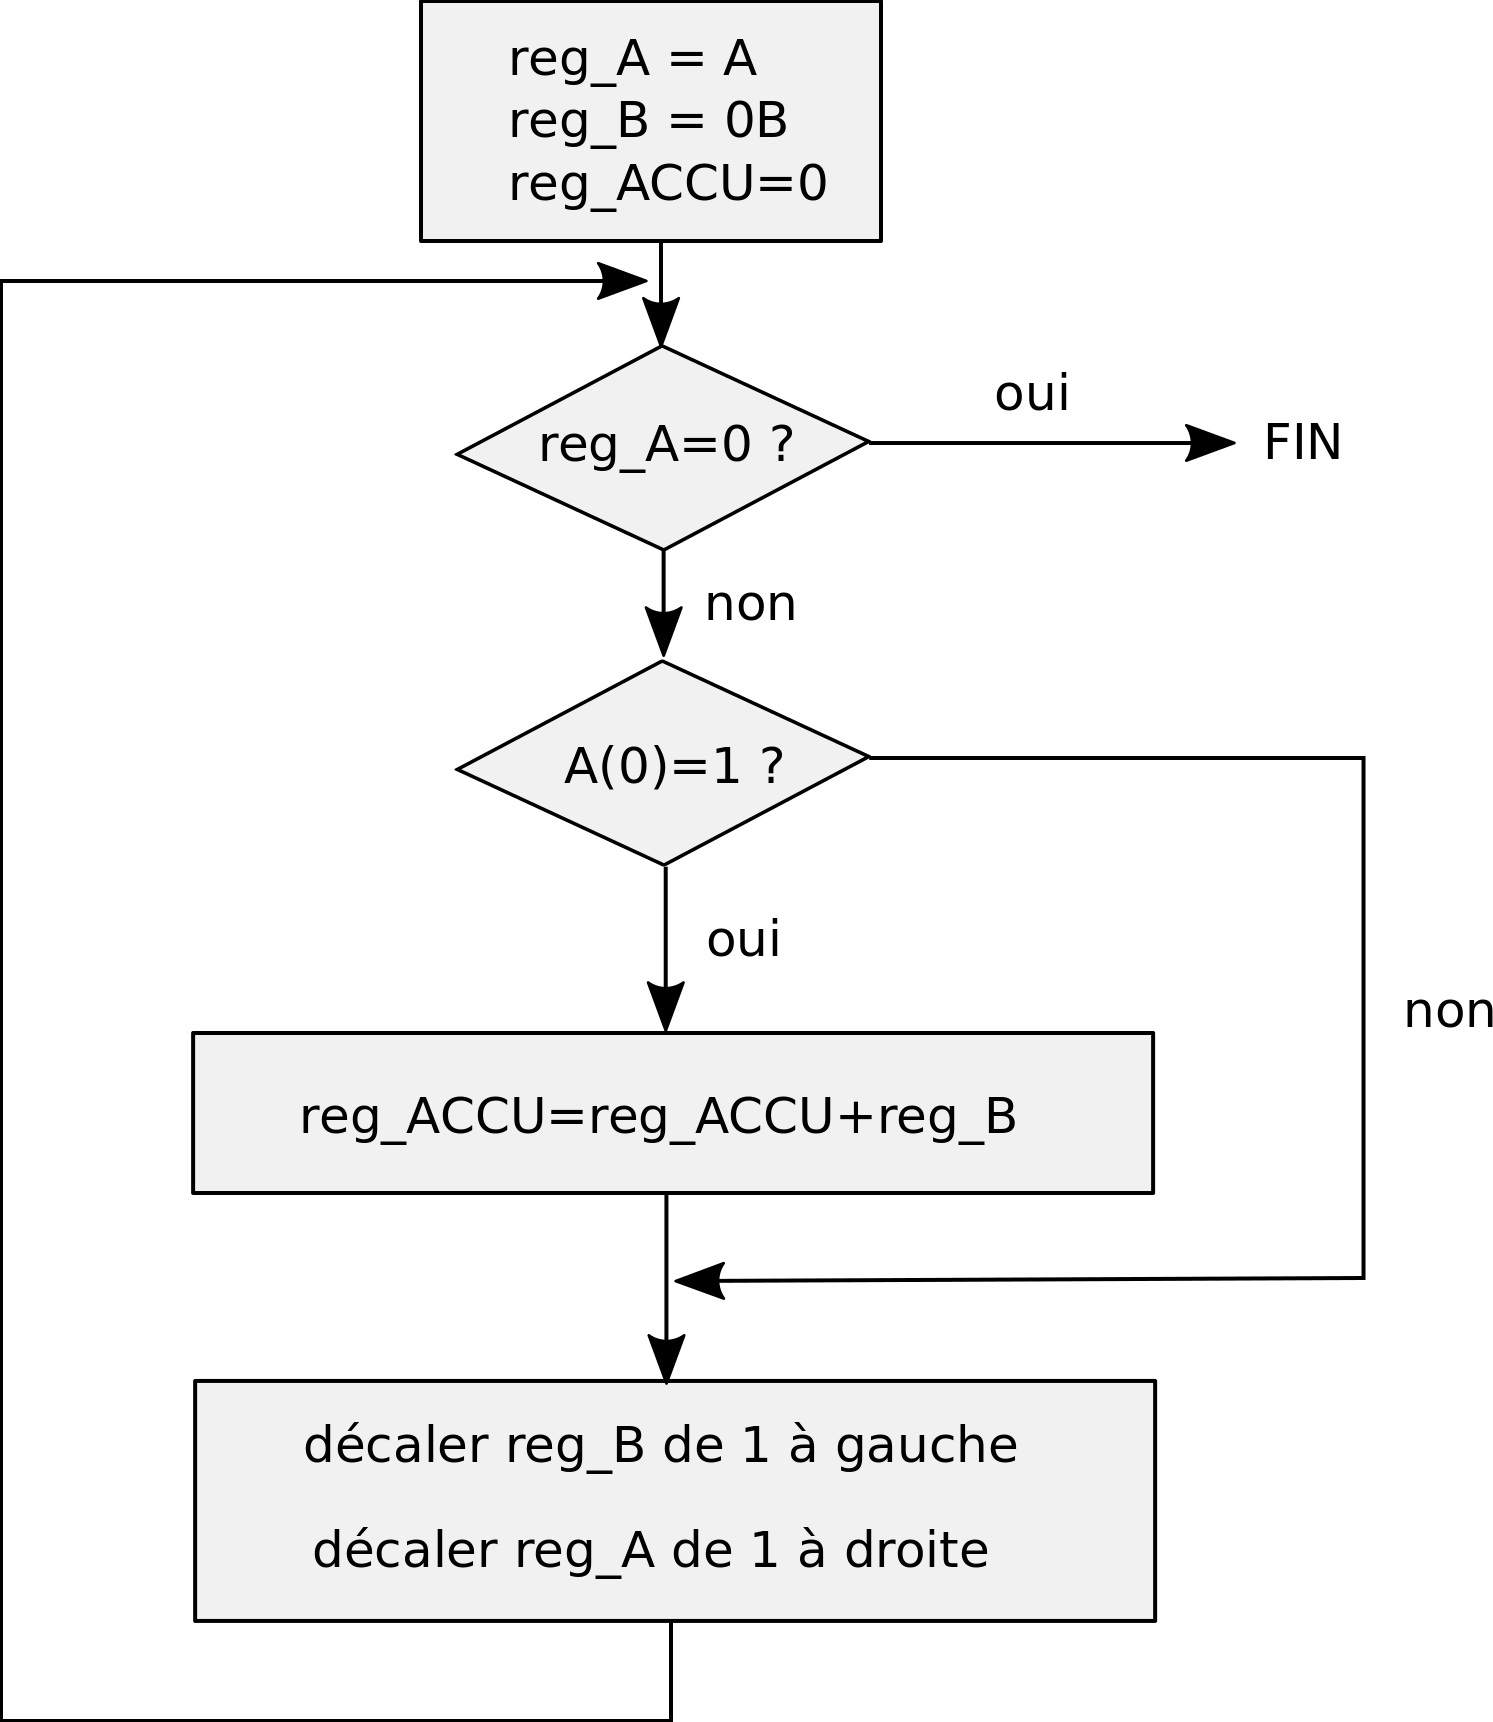
\includegraphics[scale=0.15]{./figures/flowchart.png}
\end{center}
\caption{Flowchart de l'algorithme de multiplication séquentielle}
\end{figure}
\FloatBarrier

\begin{figure}[!h]
\begin{center}
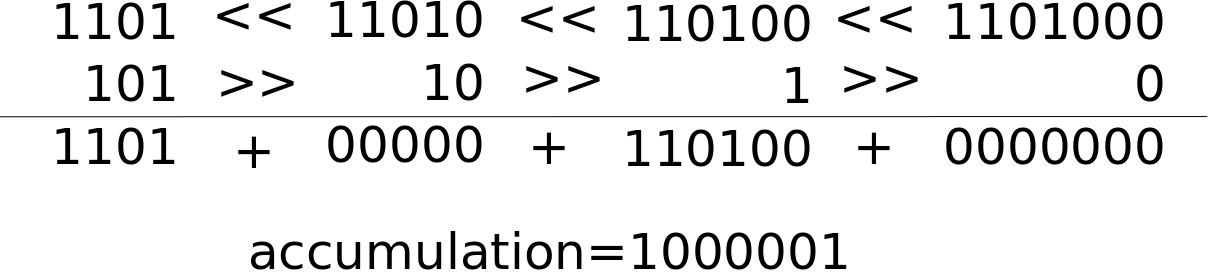
\includegraphics[scale=0.3]{./figures/algo.png}
\end{center}
\caption{Flowchart de l'algorithme de multiplication séquentielle}
\end{figure}
\FloatBarrier
%{\bf Question : } donner les différentes valeurs binaires (et décimales) des registres A, B et ACCU au cours de la multiplication pour $A=5$ et $B=13$.

\section{Décomposition FSMD}

\subsection{Rappels}
La décomposition FSMD (ou contrôleur-chemin de données) est rappelée ici, de manière générique. Le contrôleur réagit aux status du chemin de données, et contrôle ce dernier en conséquence. Le contrôleur réagit également aux ordres extérieurs (dans notre cas un 'start'), en renseigne l'extérieur sur la disponibilité des données produites (dans notre cas un signal 'end' indiquant la disponibilité du calculateur pour un nouveau calcul).

\begin{figure}[!h]
\begin{center}
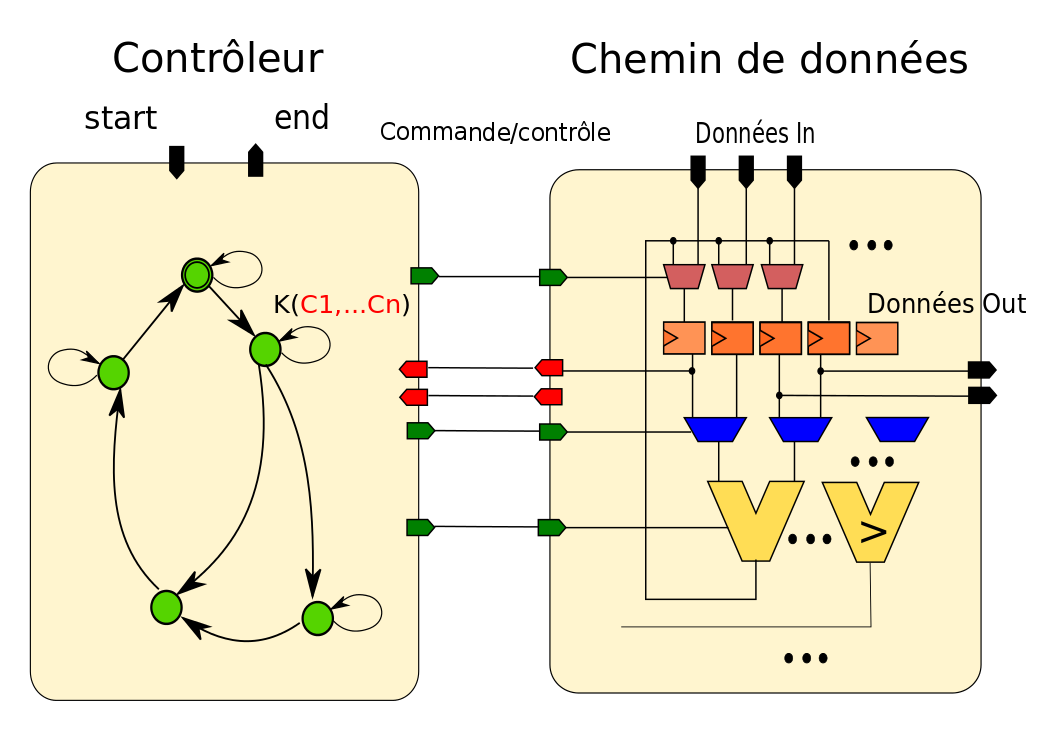
\includegraphics[scale=0.3]{./figures/FSMD-2.png}
\end{center}
\caption{Chemin de données générique}
\end{figure}
\FloatBarrier

\subsection{Chemin de données}

Les principes d'additions et de décallages successifs nous invitent à considérer 3 registres : regA, regB et ACCU qui contiendront les valeurs de A,B et de l'addition courante.

\FloatBarrier

{\bf Question 1 : }  donner les différentes valeurs binaires (et décimales) des registres regA, regB et ACCU au cours de la multiplication pour $A=5$ et $B=13$.\\

{\bf Corrections :} Cela correspond au schéma donné !

\begin{table}
    \begin{tabular}{|l|l|l|l|}
        \hline
        regA & regB     & ACCU     & cycle \\ \hline
        0101 & 00001101 & 00000000 & 1     \\ \hline
        0010 & 00011010 & 00001101 & 2     \\ \hline
        0001 & 00110100 & 00001101 & 3     \\ \hline
        0000 & 01101000 & 01000001 & 4     \\
        \hline
    \end{tabular}
\end{table}
\FloatBarrier

{\bf Question 2 : }  trouver une condition d'arrêt de cet algorithme. Cette condition constituera un élement du {\it status} renvoyé au contrôleur.\\

{\bf Corrections :} lorsqu'il n'existe plus aucun bit à 1 dans reg\_A. Pour cela il suffit de constituer le signal :

$$ stop= \overline{(reg\_A(3) + reg\_A(2) + reg\_A(1) + reg\_A(0))}$$

Le schéma suivant recense ces opérateurs, les registres ainsi que les routages (multiplexeurs) entre ces élements.

\begin{figure}[!h]
\begin{center}
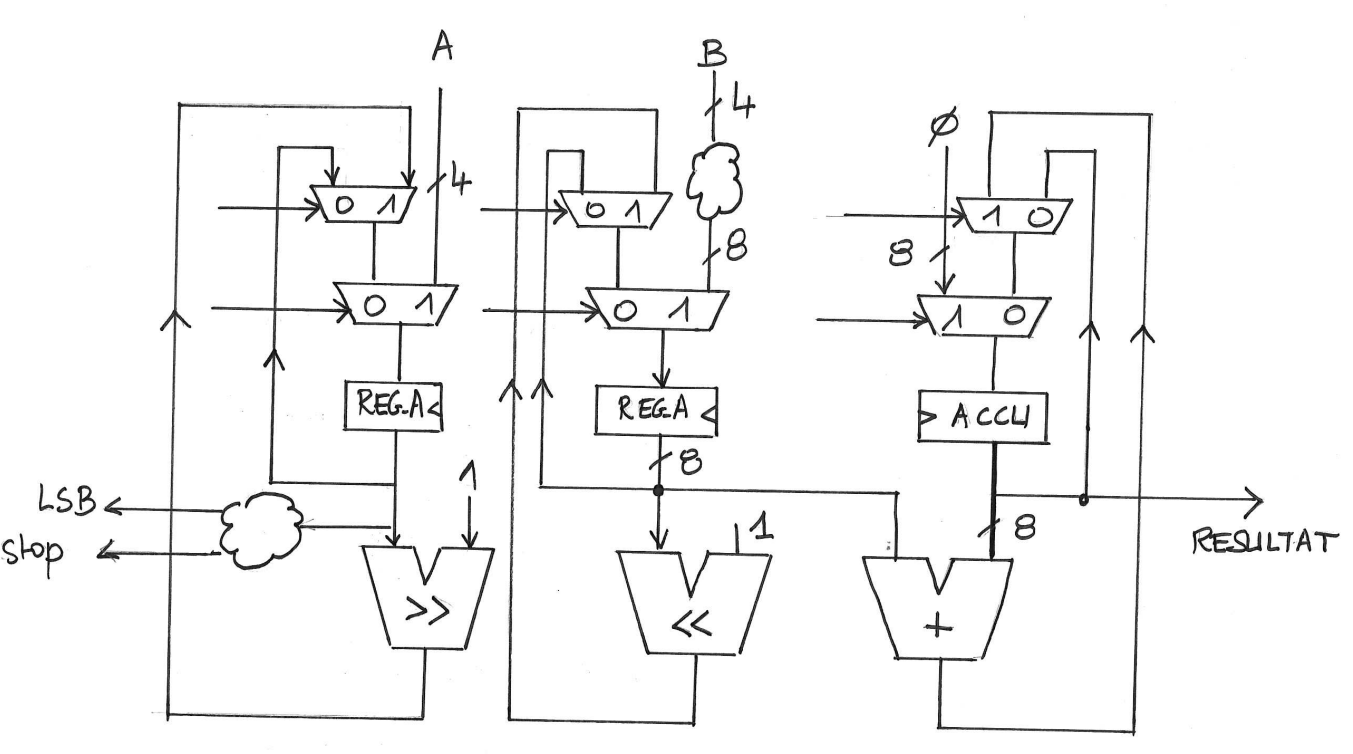
\includegraphics[scale=0.3]{./figures/datapath.png}
\end{center}
\caption{Chemin de données de l'algorithme}
\end{figure}
\FloatBarrier

{\bf Question 3 :} tenter de donner un nom significatif au signaux de contrôle des différents multiplexeurs.

{\bf Corrections :} les multiplexeurs le plus proches des entrées des registres servent à charger la donnée venant de l'extérieur, les autres servent à shifter ou additionner. {\bf Le contrôleur génère ces signaux}.

En respectant la position ``géographique'' des signaux sur le schéma, voici un nommage possible :

\begin{table}
    \begin{tabular}{|l|l|l|}
        \hline
        shift & shift & add  \\ \hline
        chA   & chB   & init \\
        \hline
    \end{tabular}
\end{table}

\subsection{Codage VHDL du chemin de données}


Sous Moodle on donne un code ``à trous'' du chemin de données. Le codage VHDL du registre regA est rappelé ici également.\\

{\bf Question 4 :} analyser ce code en tentant de faire la correspondance avec le schéma du datapath. En particulier, où se trouve le signal ``A\_Reg\_Comb'' ?\\

{\bf Solution :} ici, il faut juste tenter de comprendre l'assignation du signal  A\_Reg\_comb en VHDL : il s'agit d'une assignation conditionnelle, utilisant le mot clé ``when'' (suivi de la condition, précédée du signal ou valeur à affecter). La lecture de l'anglais doit suffire à comprendre cette assignation. Il faut comprendre que cette affectation conditionnelle correspond à un ensemble de multiplexeurs, enchaînés les uns aux autres, afin de router plusieurs donnéés ou valeurs potentielles vers l'entrée du registre (bascule D). Une écriture spécifique VHDL engendrera les circuits correspondants : c'est {\bf l'inférence matérielle}. Le signal ``A\_Reg\_Comb'' est donc situé en entrée de la bascule/registre reg\_A.\\

{\bf Question 5 :} en vous inspirant de ce code, écrire regB, puis celui d'ACCU. Pour ce dernier, vous aurez besoin d'additionner. Le type {\it unsigned} utilisé ici pour typer les registres permet effectivement d'additionner (ce n'est logiquement pas le cas de vecteurs de bits).\\

\begin{lstlisting}[caption=registre A et logique combinatoire associée, label=amb]
A_reg_proc : process (clk, reset_n)
  begin
    if reset_n = '0' then
      A_Reg <= "0000";
    elsif rising_edge(clk) then
      A_Reg <= A_Reg_comb;
    end if;
  end process;

  A_Reg_comb <= unsigned(a) when chRA = '1' else
                '0' & reg_a(3 downto 1) when shift = '1' else
                reg_a;
\end{lstlisting}

{\bf solution :}

\begin{lstlisting}[caption=registre B]
 -------------------------------------------------------------------------------
  --datatpath
  -----------------------------------------------------------------------------
  B_reg_proc : process (clk, reset_n)
  begin
    if reset_n = '0' then
      reg_b <= "00000000";
    elsif rising_edge(clk) then
      reg_b <= reg_b_comb;
    end if;
  end process;

  reg_b_comb <= unsigned("0000" & b) when chRb = '1' else
                reg_b(6 downto 0) & '0' when shift = '1' else
                reg_b;
  -----------------------------------------------------------------------------
  a_reg_proc : process (clk, reset_n)
  begin
    if reset_n = '0' then
      reg_a <= "0000";
    elsif rising_edge(clk) then
      reg_a <= reg_a_comb;
    end if;
  end process;

  reg_a_comb <= unsigned(a) when chRa = '1' else
                '0' & reg_a(3 downto 1) when shift = '1' else
                reg_a;
  -----------------------------------------------------------------------------
  ACCU : process (clk, reset_n)
  begin
    if reset_n = '0' then
      accu_reg <= unsigned(``00000000'');
    elsif rising_edge(clk) then
      accu_reg <= accu_reg_comb;
    end if;
  end process;

  accu_reg_comb <= unsigned(``00000000'') when init = '1' else
                   accu_reg + reg_b when add = '1' else
                   accu_reg;
  -----------------------------------------------------------------------------
  res <= std_logic_vector(accu_reg);

  lsb_a <= reg_a(0);
  stop  <= not(reg_a(3) or reg_a(2) or reg_a(1) or reg_a(0));

\end{lstlisting}


\subsection{Conception de l'automate}

Le diagramme à bulle de l'automate est donné ici. Les premiers états servent à attendre la fourniture des opérandes $A$ et $B$ : la présence de ces données est signalée respectivement par des signaux externes $ack_A$ et $ack_B$.

\begin{figure}[!h]
\begin{center}
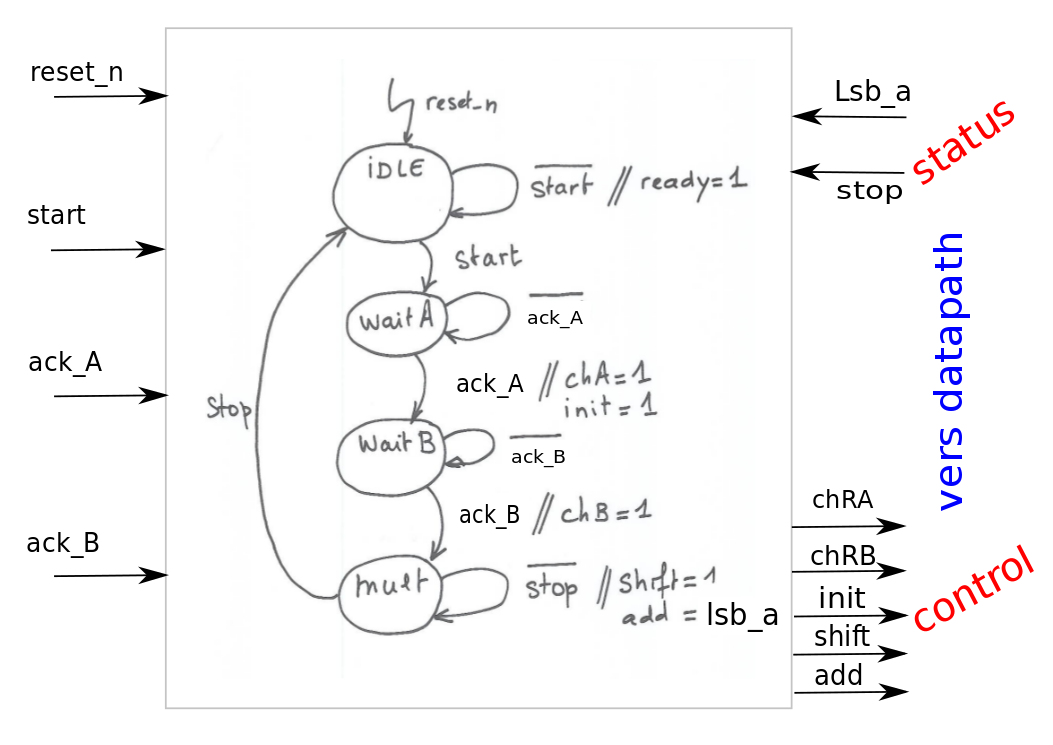
\includegraphics[scale=0.3]{./figures/controleur_fsm.png}
\end{center}
\caption{Chemin de données de l'algorithme}
\end{figure}
\FloatBarrier

{\bf Question 6 :} établir les équations de cet automate afin de contrôler le chemin de données précédent.\\

%==========================================================
{\bf solutions :} en choisissant un encodage one-hot.

Version ``à la main'', avec nom conventionnel des entrées-sorties de bascules D :

\begin{verbatim}
D0 = Q3.STOP  + Q0./START
D1 = Q0.START + Q1./ACK_A
D2 = Q1.ACK_A + Q2./ACK_B
D3 = Q2.ACK_B + Q3./STOP

SHIFT= Q3
ADD  = Q3.LSB_A
CHRA  = INIT= Q1.ACK_A
CHRB  = Q2.ACK_B
READY= Q0
\end{verbatim}

%=============================================================
{\bf Question 7 :} remplir le code à trou concernant ce contrôleur, dans le même fichier, à l'endroit prévu pour cela. En ce qui concerne le codage VHDL, inspirez vous du TE3.\\

{\bf solution :}
\begin{lstlisting}
  -----------------------------------------------------------------------------
  -- Controleur
  -----------------------------------------------------------------------------
  bascules_etat : process (clk, reset_n)
  begin
    if reset_n = '0' then
      state <= IDLE;
    elsif rising_edge(clk) then
      state <= next_state;
    end if;
  end process;

  -- logique combinatoire d'etat suivant
  next_state(0) <= (state(3) and stop) or (state(0) and not(start));
  next_state(1) <= (state(0) and start) or (state(1) and not(ack_a));
  next_state(2) <= (state(1) and ack_a) or (state(2) and not(ack_b));
  next_state(3) <= (state(2) and ack_b) or (state(3) and not(stop));

  -- signaux controleur --> datapath
  shift <= state(3);
  add   <= state(3) and lsb_a;
  chrA  <= state(1) and ack_a;
  init  <= state(1) and ack_a;
  chrB  <= state(2) and ack_b;
  -- signal vers l'exterieur (fin traitement)
  ready <= state(0);
\end{lstlisting}

\section{Simulation}

Un banc de test vous est fourni sous Moodle, qui teste le produit de $5$ par $15$.\\

{\bf Question 8 :} avec GHDL, analyser puis simuler votre circuit.

{\bf solution :} rappels. Tout ceci peut être exécuté en ligne de commande ou mis dans un fichier script sous Linux, afin d'automatiser l'exécution.
\begin{verbatim}
ghdl -a multSeq.vhd
ghdl -a multSeq_tb.vhd
ghdl -e multSeq_tb
ghdl -r multSeq_tb --wave=multseq.ghw
gtkwave multseq.ghw
\end{verbatim}

\begin{figure}[!h]
\begin{center}
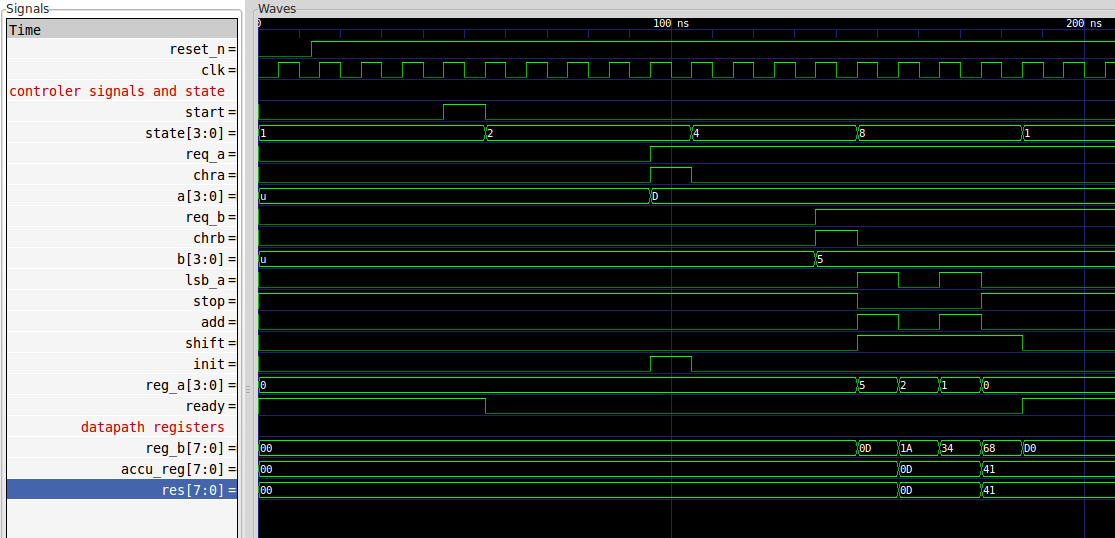
\includegraphics[scale=0.4]{./figures/wave_logic.png}
\end{center}
\caption{Forme d'onde (waveforms) dans le cas de $A=5_{10}$ et $B=13_{10}$}
\end{figure}

\section{Synthèse FPGA}

Lorsque vous avez simulé correctement, consulter votre enseignant pour observer le circuit sur plateforme FPGA Cyclone II de la société Altera, sur carte DE2.

\end{document}
